%!Mode:: "TeX:UTF-8"
\documentclass[a4paper,11pt,UTF8]{ctexart}

\usepackage{indentfirst} %缩进
\usepackage{xeCJK}    %使用系统字体
\usepackage{bm}       %粗体
\usepackage{fancyhdr} %自定义页眉页脚
\pagestyle{plain}                   %不设置页眉页脚
\usepackage{amsmath, amsthm, amssymb, amsfonts} %数学公式
\usepackage[a4paper,left=3cm,right=3cm,top=3.5cm,bottom=3.5cm]{geometry}
\usepackage{booktabs} %插入表格
\usepackage[section]{placeins} %避免浮动
\usepackage{listings} %插入代码
\usepackage{ctex}     %中文宏包
\usepackage[svgnames, table]{xcolor} %彩色表格
\usepackage{algorithm}          %伪代码
\usepackage{algorithmicx}
\usepackage{algpseudocode}
\usepackage{algorithm,algpseudocode,float}
\usepackage{lipsum}
\usepackage{enumitem}           %调整列举环境
\usepackage{url}
\usepackage{fontspec,xunicode}
\usepackage{subfigure}
\defaultfontfeatures{Mapping=tex-text} %如果没有它，会有一些 tex 特殊字符无法正常使用，比如连字符。

\usepackage{graphicx}
\graphicspath{{imgs/}}

%%%%%%%%%%%%%%%%%%%%%%%%%%%%%%%%%%%%%%%%%%%%%%%%%%%%%%%%%%%%%%%%
% 缩进及行间距
%%%%%%%%%%%%%%%%%%%%%%%%%%%%%%%%%%%%%%%%%%%%%%%%%%%%%%%%%%%%%%%%
\setlength{\parindent}{22bp} %重新定义缩进长度
\linespread{1}

%%%%%%%%%%%%%%%%%%%%%%%%%%%%%%%%%%%%%%%%%%%%%%%%%%%%%%%%%%%%%%%%
% 图的标题行间距设置
%%%%%%%%%%%%%%%%%%%%%%%%%%%%%%%%%%%%%%%%%%%%%%%%%%%%%%%%%%%%%%%%
\newcommand{\bottomcaption}{%
\setlength{\abovecaptionskip}{6bp}%
\setlength{\belowcaptionskip}{6bp}%
\caption}


%%%%%%%%%%%%%%%%%%%%%%%%%%%%%%%%%%%%%%%%%%%%%%%%%%%%%%%%%%%%%%%%
% 字体定义
%%%%%%%%%%%%%%%%%%%%%%%%%%%%%%%%%%%%%%%%%%%%%%%%%%%%%%%%%%%%%%%%
\setmainfont{Times New Roman}  %默认英文字体.serif是有衬线字体sans serif无衬线字体
\setmonofont{Consolas}
\setCJKmainfont[ItalicFont={楷体}, BoldFont={黑体}]{宋体}%衬线字体 缺省中文字体为
\setCJKsansfont{黑体}
\punctstyle{hangmobanjiao}
%-----------------------xeCJK下设置中文字体------------------------------%
\setCJKfamilyfont{song}{SimSun}                             %宋体 song
\newcommand{\song}{\CJKfamily{song}}
\setCJKfamilyfont{fs}{FangSong}                      %仿宋  fs
\newcommand{\fs}{\CJKfamily{fs}} 
\let\kaishu\relax                                    %重定义楷体，打开假粗体
\newCJKfontfamily\kaishu{KaiTi}[AutoFakeBold] 
%\setCJKfamilyfont{ktgb}{KaiTi_GB2312}                      %楷体 GB2312
%\newcommand{\ktgb}{\CJKfamily{ktgb}}
\setCJKfamilyfont{yh}{Microsoft YaHei}                    %微软雅黑 yh
\newcommand{\yh}{\CJKfamily{yh}}
\setCJKfamilyfont{hei}{SimHei}                              %黑体  hei
\newcommand{\hei}{\CJKfamily{hei}}
\setCJKfamilyfont{hwxk}{STXingkai}                                %华文行楷  hwxk
\newcommand{\hwxk}{\CJKfamily{hwxk}}
%------------------------------设置字体大小------------------------%
\newcommand{\chuhao}{\fontsize{42bp}{63bp}\selectfont}     %初号， 1.5倍行距
\newcommand{\xiaochuhao}{\fontsize{36bp}{36bp}\selectfont} %小初号，单倍行距
\newcommand{\yihao}{\fontsize{26bp}{39bp}\selectfont}        % 一号, 1.5 倍行距
\newcommand{\erhao}{\fontsize{22bp}{33bp}\selectfont}        % 二号, 1.5倍行距
\newcommand{\xiaoerhao}{\fontsize{18bp}{18bp}\selectfont}       % 小二, 单倍行距
\newcommand{\sanhao}{\fontsize{16bp}{24bp}\selectfont}       % 三号, 1.5倍行距
\newcommand{\xiaosanhao}{\fontsize{15bp}{22bp}\selectfont}      % 小三, 1.5倍行距
\newcommand{\sihao}{\fontsize{14bp}{21bp}\selectfont}        % 四号, 1.5 倍行距
\newcommand{\banxiaosi}{\fontsize{13bp}{20bp}\selectfont}  % 半小四, 20pt行距
\newcommand{\xiaosihao}{\fontsize{12bp}{20bp}\selectfont}       % 小四, 20pt行距
\newcommand{\dawuhao}{\fontsize{11bp}{11bp}\selectfont}      % 大五号, 单倍行距
\newcommand{\wuhao}{\fontsize{10.5bp}{10.5bp}\selectfont}   % 五号, 单倍行距
\newcommand{\xiaowuhao}{\fontsize{9bp}{9bp}\selectfont}   %小五号，单倍行距
%------------------------------重定义normalize------------------------%
\renewcommand{\normalsize}{\fontsize{12bp}{20bp}\selectfont}


%%%%%%%%%%%%%%%%%%%%%%%%%%%%%%%%%%%%%%%%%%%%%%%%%%%%%%%%%%%%%%%%
% 图题字体大小相同
%%%%%%%%%%%%%%%%%%%%%%%%%%%%%%%%%%%%%%%%%%%%%%%%%%%%%%%%%%%%%%%%
\usepackage{caption}
\captionsetup{font={footnotesize}}   % footnotesize = 9bp
\captionsetup[lstlisting]{font={footnotesize}}

%%%%%%%%%%%%%%%%%%%%%%%%%%%%%%%%%%%%%%%%%%%%%%%%%%%%%%%%%%%%%%%%
% 重定义枚举编号为 1),2)...
%%%%%%%%%%%%%%%%%%%%%%%%%%%%%%%%%%%%%%%%%%%%%%%%%%%%%%%%%%%%%%%%
\renewcommand{\labelenumi}{\theenumi）}


%%%%%%%%%%%%%%%%%%%%%%%%%%%%%%%%%%%%%%%%%%%%%%%%%%%%%%%%%%%%%%%%
% 重定义section标题
%%%%%%%%%%%%%%%%%%%%%%%%%%%%%%%%%%%%%%%%%%%%%%%%%%%%%%%%%%%%%%%%
\CTEXsetup[format={\CJKfamily{zhhei}\zihao{4}},number={\chinese{section}},name={,、~},aftername={},indent={0bp},beforeskip={6bp},afterskip={6bp},format+={\flushleft}]{section}
% \CTEXsetup[format={\Large\bfseries\CJKfamily{zhkai}\zihao{5}},name={（,）},number={\chinese{subsection}},aftername={},indent={22bp},beforeskip={6bp},afterskip={6bp}]{subsection}
\CTEXsetup[number={\chinese{section}},name={附录, ~~ }]{appendix}



%%%%%%%%%%%%%%%%%%%%%%%%%%%%%%%%%%%%%%%%%%%%%%%%%%%%%%%%%%%%%%%%
% 标题名称中文化
%%%%%%%%%%%%%%%%%%%%%%%%%%%%%%%%%%%%%%%%%%%%%%%%%%%%%%%%%%%%%%%%
\renewcommand\figurename{\hei 图}
\renewcommand\tablename{\hei 表}
\renewcommand\lstlistingname{\hei 代码}
\renewcommand{\algorithmicrequire}{\textbf{输入:}}
\renewcommand{\algorithmicensure}{\textbf{输出:}}
\newtheorem{define}{定义}


%%%%%%%%%%%%%%%%%%%%%%%%%%%%%%%%%%%%%%%%%%%%%%%%%%%%%%%%%%%%%%%%
% 列表设置
%%%%%%%%%%%%%%%%%%%%%%%%%%%%%%%%%%%%%%%%%%%%%%%%%%%%%%%%%%%%%%%%
\setlist[enumerate,1]{itemindent=22bp,listparindent=\parindent,itemsep=0mm,partopsep=.7mm,parsep=0ex,labelsep=1.5mm,topsep=0.7mm}
\setlist[enumerate,2]{label=\alph*),leftmargin=1.5em}  %二级item设置
%\setitemize{itemindent=38bp,leftmargin=0bp,itemsep=-0.4ex,listparindent=26bp,partopsep=0bp,parsep=0.5ex,topsep=-0.25ex}
%\setdescription{itemindent=38bp,leftmargin=0bp,itemsep=-0.4ex,listparindent=26bp,partopsep=0bp,parsep=0.5ex,topsep=-0.25ex}

%%%%%%%%%%%%%%%%%%%%%%%%%%%%%%%%%%%%%%%%%%%%%%%%%%%%%%%%%%%%%%%%
% 代码设置
%%%%%%%%%%%%%%%%%%%%%%%%%%%%%%%%%%%%%%%%%%%%%%%%%%%%%%%%%%%%%%%%
\lstset{
 columns=fixed,
 numbers=left,                                        % 在左侧显示行号
 numberstyle=\tiny\color{gray},                       % 设定行号格式
 frame=single,                                        % 单线背景边框
 breaklines=true,                                     % 设定LaTeX对过长的代码行进行自动换行
 keywordstyle=\color[RGB]{40,40,255},                 % 设定关键字颜色
 numberstyle=\footnotesize\color{darkgray},
 commentstyle=\it\color[RGB]{0,96,96},                % 设置代码注释的格式
 stringstyle=\rmfamily\slshape\color[RGB]{128,0,0},   % 设置字符串格式
 showstringspaces=false,                              % 不显示字符串中的空格
 language=java,                                        % 设置语言
 basicstyle=\linespread{1.0}\xiaowuhao\ttfamily,                      % 字体字号
 %lineskip=10bp,
 %baselinestretch=1,
}

%%%%%%%%%%%%%%%%%%%%%%%%%%%%%%%%%%%%%%%%%%%%%%%%%%%%%%%%%%%%%%%%
% 伪代码分页
%%%%%%%%%%%%%%%%%%%%%%%%%%%%%%%%%%%%%%%%%%%%%%%%%%%%%%%%%%%%%%%%
\makeatletter
\renewcommand{\ALG@name}{算法}
\newenvironment{breakablealgorithm}
  {% \begin{breakablealgorithm}
   \begin{center}
     \refstepcounter{algorithm}% New algorithm
     \hrule height.8bp depth0bp \kern2bp% \@fs@pre for \@fs@ruled
     \renewcommand{\caption}[2][\relax]{% Make a new \caption
       {\raggedright\textbf{\ALG@name~\thealgorithm} ##2\par}%
       \ifx\relax##1\relax % #1 is \relax
         \addcontentsline{loa}{algorithm}{\protect\numberline{\thealgorithm}##2}%
       \else % #1 is not \relax
         \addcontentsline{loa}{algorithm}{\protect\numberline{\thealgorithm}##1}%
       \fi
       \kern2bp\hrule\kern2bp
     }
  }{% \end{breakablealgorithm}
     \kern2bp\hrule\relax% \@fs@post for \@fs@ruled
   \end{center}
  }
\makeatother



\begin{document}
\xiaosihao\song

\begin{titlepage}
\center{\yihao{\hwxk{电子科技大学\underline{自动化}学院}}}
\vspace{6cm}
\center{\xiaochuhao{\kaishu{\bfseries 实~验~报~告}}}
\vspace{4cm}

\begin{center}
\begin{large}
\begin{tabular}{rc}
\xiaoerhao{\hei{学\qquad 号}}& \hspace{1.7cm}\xiaoerhao{\hei{202422080235\hspace{1.7cm}}} \\
\cline{2-2}\\
\xiaoerhao{\hei{姓\qquad 名}}& \xiaoerhao{\hei{李皓}}\\
\cline{2-2}\\
\xiaoerhao{\hei{（实验）课程名称}}& \xiaoerhao{\hei{实验二~模糊图像复原}}\\
\cline{2-2}\\
\xiaoerhao{\hei{教师}}& \xiaoerhao{\hei{于力}}\\
\cline{2-2}\\

\end{tabular}
\end{large}
\end{center}
\vfill \hfill
\end{titlepage}
\clearpage

\centerline{\\[10bp]\erhao{\fs{电 ~子 ~科~ 技~ 大~ 学}}}

\centerline{\\[20bp]\yihao{\fs{实  ~~~~ 验  ~~~~ 报  ~~~~ 告}}}

\leftline{\\[10bp]\sihao{\hei{\hspace{1.5em} 学生姓名：李皓 \hfill 学号：202422080235 \hfill 指导教师：于力 }}}

% \leftline{\\[10bp]\sihao{\hei{\hspace{1.5em} 实验地点：信软楼西XXX \hfill }}}

% \leftline{\\[10bp]\sihao{\hei{\hspace{1.5em} 实验时间：第X周周X（X-X节） \hfill }}}

\setlength{\parskip}{0bp}  %定义段间距

\section{实验名称：模糊图像复原}

\section{实验目的:}
\begin{enumerate}
    \item 理解并掌握维纳滤波在图像复原中的原理与实现
    \item 学习不同噪声核的估计方法，包括频谱分析、梯度分析、Radon变换和盲反卷积
    \item 比较分析不同噪声核估计方法对模糊图像复原效果的影响
    \item 探究维纳滤波参数对复原效果的影响，并学习自动优化参数的方法
\end{enumerate}

\section{实验原理:}
\subsection{图像模糊与退化模型}
图像的模糊过程可以通过线性系统的退化模型来描述。设原始清晰图像为$f(x,y)$，模糊后的图像为$g(x,y)$，则退化过程可表示为：
\begin{equation}
g(x,y) = h(x,y) * f(x,y) + n(x,y)
\end{equation}

其中，$h(x,y)$是点扩散函数(PSF)，表示模糊核；$*$表示卷积操作；$n(x,y)$是加性噪声。在频域中，上述模型可表示为：
\begin{equation}
G(u,v) = H(u,v) \cdot F(u,v) + N(u,v)
\end{equation}

图像复原的目标是在已知$g(x,y)$和$h(x,y)$（或估计出$h(x,y)$）的情况下，恢复出接近原始图像$f(x,y)$的图像。

\subsection{维纳滤波 (Wiener Filter)}
维纳滤波是一种基于最小均方误差准则的复原方法，考虑了图像和噪声的统计特性。其频域表达式为：
\begin{equation}
W(u,v) = \frac{H^*(u,v)}{|H(u,v)|^2 + K}
\end{equation}

其中，$H^*(u,v)$是$H(u,v)$的复共轭，$K$是一个常数，与信噪比相关：$K = \frac{S_n(u,v)}{S_f(u,v)}$，其中$S_n$和$S_f$分别是噪声和原始图像的功率谱密度。实际应用中，$K$通常作为一个可调参数。

复原过程为：
\begin{equation}
\hat{F}(u,v) = W(u,v) \cdot G(u,v)
\end{equation}

\subsection{运动模糊核的估计方法}
运动模糊是图像退化的常见形式，由相机或物体在曝光过程中的相对运动引起。对于匀速线性运动，其模糊核可以用以下模型表示：
\begin{equation}
h(x,y) = 
\begin{cases}
\frac{1}{L}, & \text{如果} \sqrt{x^2 + y^2} \leq \frac{L}{2} \text{且} \frac{x}{y} = \frac{\cos\theta}{\sin\theta} \\
0, & \text{其他情况}
\end{cases}
\end{equation}

其中，$L$是模糊长度，$\theta$是模糊方向。准确估计这两个参数对图像复原至关重要。以下介绍四种主要的估计方法：

\subsubsection{频谱分析法}
频谱分析法基于模糊图像的傅里叶变换特性。在频域中，运动模糊表现为沿垂直于运动方向的条纹状结构。这源于运动模糊核在频域的表达式：

\begin{equation}
H(u,v) = \frac{\sin[\pi(u\cos\theta + v\sin\theta)L]}{\pi(u\cos\theta + v\sin\theta)L} \cdot e^{-j\pi(u\cos\theta + v\sin\theta)L}
\end{equation}

其中$u$和$v$为频域坐标。由于$\text{sinc}$函数的特性，$H(u,v)$会在垂直于运动方向的频率上出现周期性的零点，形成可见的条纹。

具体步骤包括：
\begin{enumerate}
    \item 对模糊图像进行傅里叶变换：$F(u,v) = \mathcal{F}\{g(x,y)\}$
    \item 计算幅值谱并取对数增强可视性：$M(u,v) = \log(|F(u,v)| + 1)$
    \item 对幅值谱进行归一化和阈值处理：
    \begin{equation}
    M_{\text{norm}}(u,v) = \frac{M(u,v) - \min(M)}{\max(M) - \min(M)} \cdot 255
    \end{equation}
    \begin{equation}
    M_{\text{thresh}}(u,v) = 
    \begin{cases}
    255, & \text{如果} M_{\text{norm}}(u,v) < T \\
    0, & \text{否则}
    \end{cases}
    \end{equation}
    其中$T$是阈值，通常取127
    \item 使用霍夫变换检测线条：
    \begin{equation}
    \rho = x\cos\phi + y\sin\phi
    \end{equation}
    每条线由参数$(\rho, \phi)$表示
    \item 计算主要线条方向的平均值，模糊方向通常垂直于此：
    \begin{equation}
    \theta_{\text{motion}} = (\phi_{\text{avg}} - 90^\circ) \mod 180^\circ
    \end{equation}
    \item 根据频谱中零点之间的距离估计模糊长度：
    \begin{equation}
    L \approx \frac{1}{\Delta f}
    \end{equation}
    其中$\Delta f$是相邻零点间的频率间隔
\end{enumerate}

\subsubsection{梯度分析法}
梯度分析法基于这样一个观察：运动模糊使垂直于运动方向的边缘保持较为清晰，而沿运动方向的边缘变得模糊。因此，图像梯度主要分布在垂直于运动方向的方向上。

设模糊图像为$g(x,y)$，其梯度可表示为：
\begin{equation}
\nabla g(x,y) = \left(\frac{\partial g}{\partial x}, \frac{\partial g}{\partial y}\right) = (g_x, g_y)
\end{equation}

梯度方向和强度可以计算为：
\begin{equation}
\phi(x,y) = \arctan\left(\frac{g_y}{g_x}\right)
\end{equation}
\begin{equation}
|\nabla g(x,y)| = \sqrt{g_x^2 + g_y^2}
\end{equation}

具体步骤包括：
\begin{enumerate}
    \item 使用Sobel算子计算$x$和$y$方向的梯度：
    \begin{equation}
    g_x = S_x * g, \quad g_y = S_y * g
    \end{equation}
    其中$S_x$和$S_y$分别是$x$和$y$方向的Sobel算子
    \item 计算梯度方向直方图，以梯度强度为权重：
    \begin{equation}
    H(\phi_i) = \sum_{x,y} |\nabla g(x,y)| \cdot \delta(\phi(x,y) - \phi_i)
    \end{equation}
    其中$\delta$是狄拉克函数，表示当条件满足时为1，否则为0
    \item 找出梯度方向直方图中的峰值，确定主要梯度方向$\phi_{\text{main}}$
    \item 运动方向与主梯度方向正交：
    \begin{equation}
    \theta_{\text{motion}} = (\phi_{\text{main}} + 90^\circ) \mod 180^\circ
    \end{equation}
    \item 使用自相关分析估计模糊长度。在运动方向上计算图像的自相关函数：
    \begin{equation}
    R(d) = \sum_{x,y} g(x,y) \cdot g(x+d\cos\theta_{\text{motion}}, y+d\sin\theta_{\text{motion}})
    \end{equation}
    分析$R(d)$的衰减特性可估计模糊长度$L$
\end{enumerate}

\subsubsection{Radon变换法}
Radon变换将二维图像转换为一系列沿不同角度的一维投影。设图像为$g(x,y)$，其Radon变换可表示为：
\begin{equation}
\mathcal{R}g(\rho, \phi) = \int_{-\infty}^{\infty}\int_{-\infty}^{\infty} g(x,y) \delta(\rho - x\cos\phi - y\sin\phi) \, dx \, dy
\end{equation}

其中$\rho$是从原点到线的垂直距离，$\phi$是线的角度。对于运动模糊图像，沿运动方向的投影会产生较高的方差。

具体步骤包括：
\begin{enumerate}
    \item 对模糊图像进行边缘检测，得到边缘图像$e(x,y)$：
    \begin{equation}
    e(x,y) = \text{Canny}(g(x,y), \text{threshold}_{\text{low}}, \text{threshold}_{\text{high}})
    \end{equation}
    \item 对边缘图像进行Radon变换：
    \begin{equation}
    \mathcal{R}e(\rho, \phi) = \int_{-\infty}^{\infty}\int_{-\infty}^{\infty} e(x,y) \delta(\rho - x\cos\phi - y\sin\phi) \, dx \, dy
    \end{equation}
    \item 计算每个角度$\phi$下投影的方差：
    \begin{equation}
    V(\phi) = \text{Var}[\mathcal{R}e(\rho, \phi)]_{\rho}
    \end{equation}
    \item 找出方差最大的角度，该角度对应于垂直于运动方向的线：
    \begin{equation}
    \phi_{\text{max}} = \underset{\phi}{\operatorname{argmax}} \, V(\phi)
    \end{equation}
    \item 运动方向与此垂直：
    \begin{equation}
    \theta_{\text{motion}} = (\phi_{\text{max}} + 90^\circ) \mod 180^\circ
    \end{equation}
    \item 使用最大方差的大小估计模糊长度：
    \begin{equation}
    L \approx \alpha \cdot V(\phi_{\text{max}})
    \end{equation}
    其中$\alpha$是一个与图像大小相关的缩放因子
\end{enumerate}

\subsubsection{盲反卷积法}
盲反卷积是一种迭代优化方法，同时估计原始图像$f(x,y)$和模糊核$h(x,y)$。从数学角度看，盲反卷积可以表述为以下优化问题：
\begin{equation}
\min_{f,h} \|h * f - g\|^2 + \lambda_f R_f(f) + \lambda_h R_h(h)
\end{equation}

其中$R_f$和$R_h$分别是对原始图像和模糊核的正则化项，$\lambda_f$和$\lambda_h$是相应的权重参数。

简化的盲反卷积算法如下：
\begin{enumerate}
    \item 初始化模糊核$h^{(0)}(x,y)$，通常假设为一个简单的形状，如一条线段
    \item 迭代优化：对于迭代步骤$t = 0, 1, 2, ...$
    \begin{enumerate}
        \item 固定当前的核$h^{(t)}$，估计原始图像$f^{(t+1)}$：
        \begin{equation}
        f^{(t+1)} = \underset{f}{\operatorname{argmin}} \|h^{(t)} * f - g\|^2 + \lambda_f R_f(f)
        \end{equation}
        这一步通常使用维纳滤波或其他反卷积方法
        \item 固定当前的图像估计$f^{(t+1)}$，更新模糊核$h^{(t+1)}$：
        \begin{equation}
        h^{(t+1)} = \underset{h}{\operatorname{argmin}} \|h * f^{(t+1)} - g\|^2 + \lambda_h R_h(h)
        \end{equation}
        这一步通常涉及约束优化，确保模糊核非负且总和为1
        \item 为减少噪声影响，通常对$f^{(t+1)}$进行边缘提取，用于下一迭代的核估计
    \end{enumerate}
    \item 当达到最大迭代次数或收敛条件时停止
    \item 分析最终估计的模糊核$h$，提取模糊长度$L$和方向$\theta$
\end{enumerate}

盲反卷积是一个病态问题，存在多个局部最优解。为提高算法稳定性，通常采用多尺度策略、边缘先验和稀疏性约束等技术。虽然计算复杂度高，但它在没有先验信息的情况下通常能提供较好的估计结果。

实际实现中，Richardson-Lucy算法是一种常用的盲反卷积方法，其迭代公式为：
\begin{equation}
f^{(t+1)} = f^{(t)} \cdot \left[h^{(t)} * \left(\frac{g}{h^{(t)} * f^{(t)}}\right)\right]
\end{equation}
其中$*$表示卷积，$\cdot$表示元素乘法，分式表示元素除法。

\section{实验内容:}
本实验实现并对比了四种运动模糊核估计方法，并使用维纳滤波进行图像复原。实验包括以下内容：
\begin{enumerate}
    \item 实现四种运动模糊核估计方法：频谱分析法、梯度分析法、Radon变换法和盲反卷积法
    \item 使用估计的模糊核，结合维纳滤波进行图像复原
    \item 比较不同方法的复原效果，并分析评价指标
    \item 自动调优维纳滤波参数，探索最佳复原效果
\end{enumerate}

\section{实验设备:}
\begin{itemize}
    \item 硬件: i5-13500，32GB RAM
    \item 软件: Python 3.11, OpenCV, NumPy, SciPy, Matplotlib, scikit-image等
\end{itemize}

\section{实验步骤:}
\subsection{模糊核估计与图像复原}
\begin{enumerate}
    \item 读取模糊图像，并准备不同的模糊核估计方法
    \item 使用四种方法分别估计运动模糊参数（长度和角度）
    \item 根据估计的参数生成对应的模糊核
    \item 对图像的RGB三个通道分别应用维纳滤波
    \item 合并处理后的通道，得到复原图像
    \item 保存各种方法的复原结果
\end{enumerate}

核心代码实现:
\begin{lstlisting}[language=Python]
def wiener_filter(img, kernel, K=0.01):
    """应用维纳滤波去除图像模糊"""
    # 转换为浮点数
    img = img.astype(float)
    kernel = kernel.astype(float)
    
    # 确保核的和为1
    if np.sum(kernel) != 0:
        kernel = kernel / np.sum(kernel)
    
    # 计算图像的傅里叶变换
    img_fft = fftpack.fft2(img)
    
    # 为核填充0使其与图像大小相同
    kernel_padded = np.zeros_like(img)
    kh, kw = kernel.shape
    kernel_padded[:kh, :kw] = kernel
    
    # 确保核居中
    kernel_padded = np.roll(kernel_padded, -kh//2, axis=0)
    kernel_padded = np.roll(kernel_padded, -kw//2, axis=1)
    
    # 计算PSF的傅里叶变换
    kernel_fft = fftpack.fft2(kernel_padded)
    
    # 维纳滤波公式
    kernel_fft_conj = np.conj(kernel_fft)
    denominator = np.abs(kernel_fft)**2 + K
    wiener_filter = kernel_fft_conj / denominator
    
    # 应用滤波器
    img_deconvolved = wiener_filter * img_fft
    
    # 反变换获取结果
    img_restored = np.abs(fftpack.ifft2(img_deconvolved))
    
    # 限制像素值范围为[0, 255]
    img_restored = np.clip(img_restored, 0, 255)
    
    return img_restored.astype(np.uint8)
\end{lstlisting}

\subsection{频谱分析法估计模糊核}
\begin{lstlisting}[language=Python]
def estimate_motion_blur_spectrum(blurred_img):
    """使用频谱分析估计运动模糊参数"""
    # 转为灰度图
    if len(blurred_img.shape) == 3:
        gray = cv2.cvtColor(blurred_img, cv2.COLOR_BGR2GRAY)
    else:
        gray = blurred_img.copy()
    
    # 计算傅里叶变换
    f = np.fft.fft2(gray)
    fshift = np.fft.fftshift(f)
    magnitude_spectrum = np.log(np.abs(fshift) + 1)
    
    # 归一化频谱以增强对比度
    magnitude_spectrum_norm = (magnitude_spectrum - np.min(magnitude_spectrum)) / (np.max(magnitude_spectrum) - np.min(magnitude_spectrum)) * 255
    magnitude_spectrum_norm = magnitude_spectrum_norm.astype(np.uint8)
    
    # 应用阈值处理，以突显低频区域中的线型特征
    _, thresh = cv2.threshold(magnitude_spectrum_norm, 127, 255, cv2.THRESH_BINARY_INV)
    
    # 使用霍夫变换检测线条
    lines = cv2.HoughLines(thresh, 1, np.pi/180, 50)
    
    if lines is not None and len(lines) > 0:
        # 计算所有线的平均值
        sum_angle = 0
        count = 0
        
        for line in lines:
            rho, theta = line[0]
            # 转换角度确保在0-180度范围内
            angle_deg = (theta * 180 / np.pi) % 180
            
            # 只考虑接近垂直于运动方向的线
            if 45 <= angle_deg <= 135:
                sum_angle += angle_deg
                count += 1
        
        if count > 0:
            # 计算平均角度，然后旋转90度得到运动方向
            avg_angle = sum_angle / count
            motion_angle = (avg_angle - 90) % 180
            
            # 根据频谱中线的长度估计模糊核的长度
            line_length = min(40, max(5, thresh.shape[0] // 15))
            
            return line_length, motion_angle
    
    # 默认返回值
    return 10, 0
\end{lstlisting}

\subsection{自动调优维纳滤波参数}
\begin{lstlisting}[language=Python]
def auto_tune_deblur(img, kernels, kernel_names):
    """尝试不同的去模糊参数并选择最佳结果"""
    print("\n自动调整去模糊参数...")
    
    best_result = None
    best_score = -float('inf')
    best_params = None
    
    # 灰度图用于评估
    if len(img.shape) == 3:
        gray = cv2.cvtColor(img, cv2.COLOR_BGR2GRAY)
    else:
        gray = img.copy()
    
    # 尝试不同的K值（维纳滤波参数）
    k_values = [0.001, 0.005, 0.01, 0.02, 0.05]
    
    best_k_per_method = []
    
    for i, (kernel, name) in enumerate(zip(kernels, kernel_names)):
        best_k_score = -float('inf')
        best_k_value = 0.01
        best_k_result = None
        
        for k in k_values:
            if len(img.shape) == 3:
                b, g, r = cv2.split(img)
                b_restored = wiener_filter(b, kernel, k)
                g_restored = wiener_filter(g, kernel, k)
                r_restored = wiener_filter(r, kernel, k)
                result = cv2.merge([b_restored, g_restored, r_restored])
                # 转为灰度用于评估
                result_gray = cv2.cvtColor(result, cv2.COLOR_BGR2GRAY)
            else:
                result = wiener_filter(img, kernel, k)
                result_gray = result
            
            # 确保结果图像和原始灰度图的尺寸相同
            if result_gray.shape != gray.shape:
                result_gray = cv2.resize(result_gray, (gray.shape[1], gray.shape[0]))
            
            # 计算各种指标
            psnr_val = psnr(gray, result_gray)
            ssim_val = ssim(gray, result_gray)
            edges = cv2.Canny(result_gray.astype(np.uint8), 100, 200)
            edge_strength = np.sum(edges) / (edges.shape[0] * edges.shape[1])
            
            # 计算综合得分
            score = (
                psnr_val / 50.0 * 0.3 +   # 标准化PSNR
                ssim_val * 0.4 +          # SSIM已在0-1之间
                edge_strength / 0.1 * 0.3  # 标准化边缘强度
            )
            
            if score > best_k_score:
                best_k_score = score
                best_k_value = k
                best_k_result = result
        
        print(f"{name} 的最佳K值: {best_k_value}, 得分: {best_k_score:.4f}")
        best_k_per_method.append((best_k_value, best_k_score, best_k_result))
        
        # 更新全局最佳
        if best_k_score > best_score:
            best_score = best_k_score
            best_result = best_k_result
            best_params = (name, best_k_value)
    
    return best_result, best_params
\end{lstlisting}

\section{实验结果与分析:}
\subsection{模糊核估计结果}
实验中对一张模糊图像使用四种不同的方法进行了模糊核参数估计，结果如下：

\begin{figure}[htbp]
  \centering
  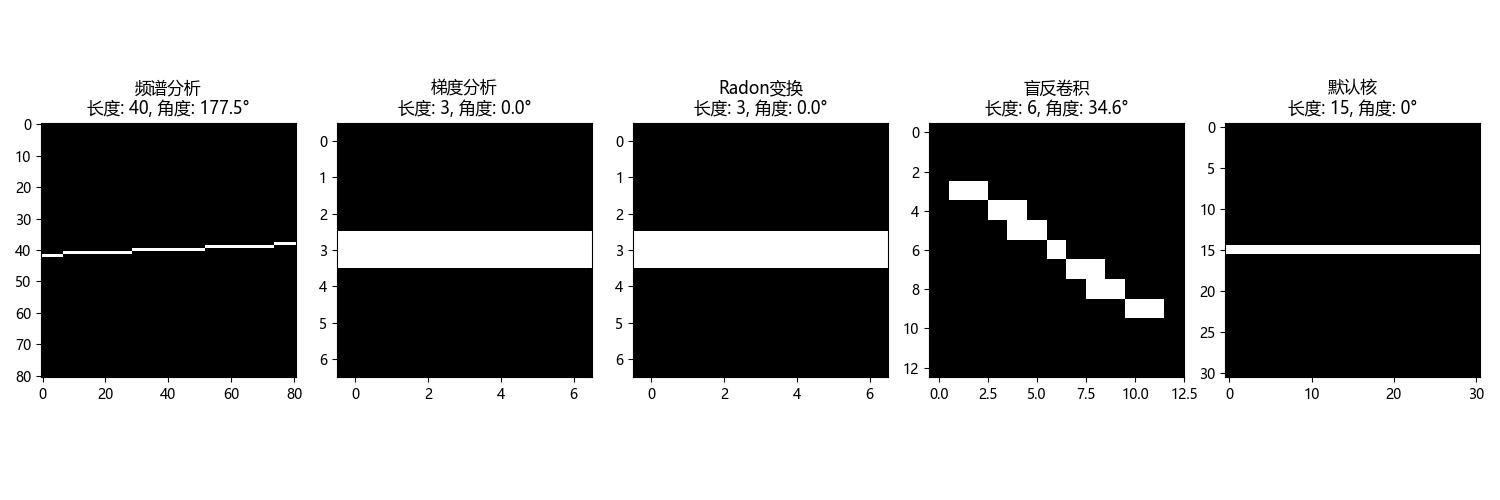
\includegraphics[width=0.9\textwidth]{2.kernels_comparison.jpg}
  \caption{不同方法估计的模糊核对比}
\end{figure}

如图1所示，四种方法估计出的模糊核在形状和方向上存在明显差异：
\begin{itemize}
    \item 频谱分析法估计的模糊核长度为40，角度为177.5度，基本呈水平方向
    \item 梯度分析法估计的模糊核长度为3，角度约为0度，形成水平方向
    \item Radon变换法估计的模糊核长度为3，角度约为0度，和梯度分析一致
    \item 盲反卷积法估计的模糊核长度为6，角度约为34.6度，倾斜程度最大
\end{itemize}
此外，还设置了长度为 15，角度为0的默认核作为对比。

这些差异主要源于各种方法对图像特征的不同侧重和处理策略。频谱分析法依赖于傅里叶域中的条纹特征，梯度分析法关注边缘的梯度分布，Radon变换法基于图像的投影特性，而盲反卷积法则通过迭代优化同时估计图像和模糊核。

\subsection{图像复原结果}
使用不同方法估计的模糊核，结合维纳滤波进行图像复原，结果如下：

\begin{figure}[htbp]
  \centering
  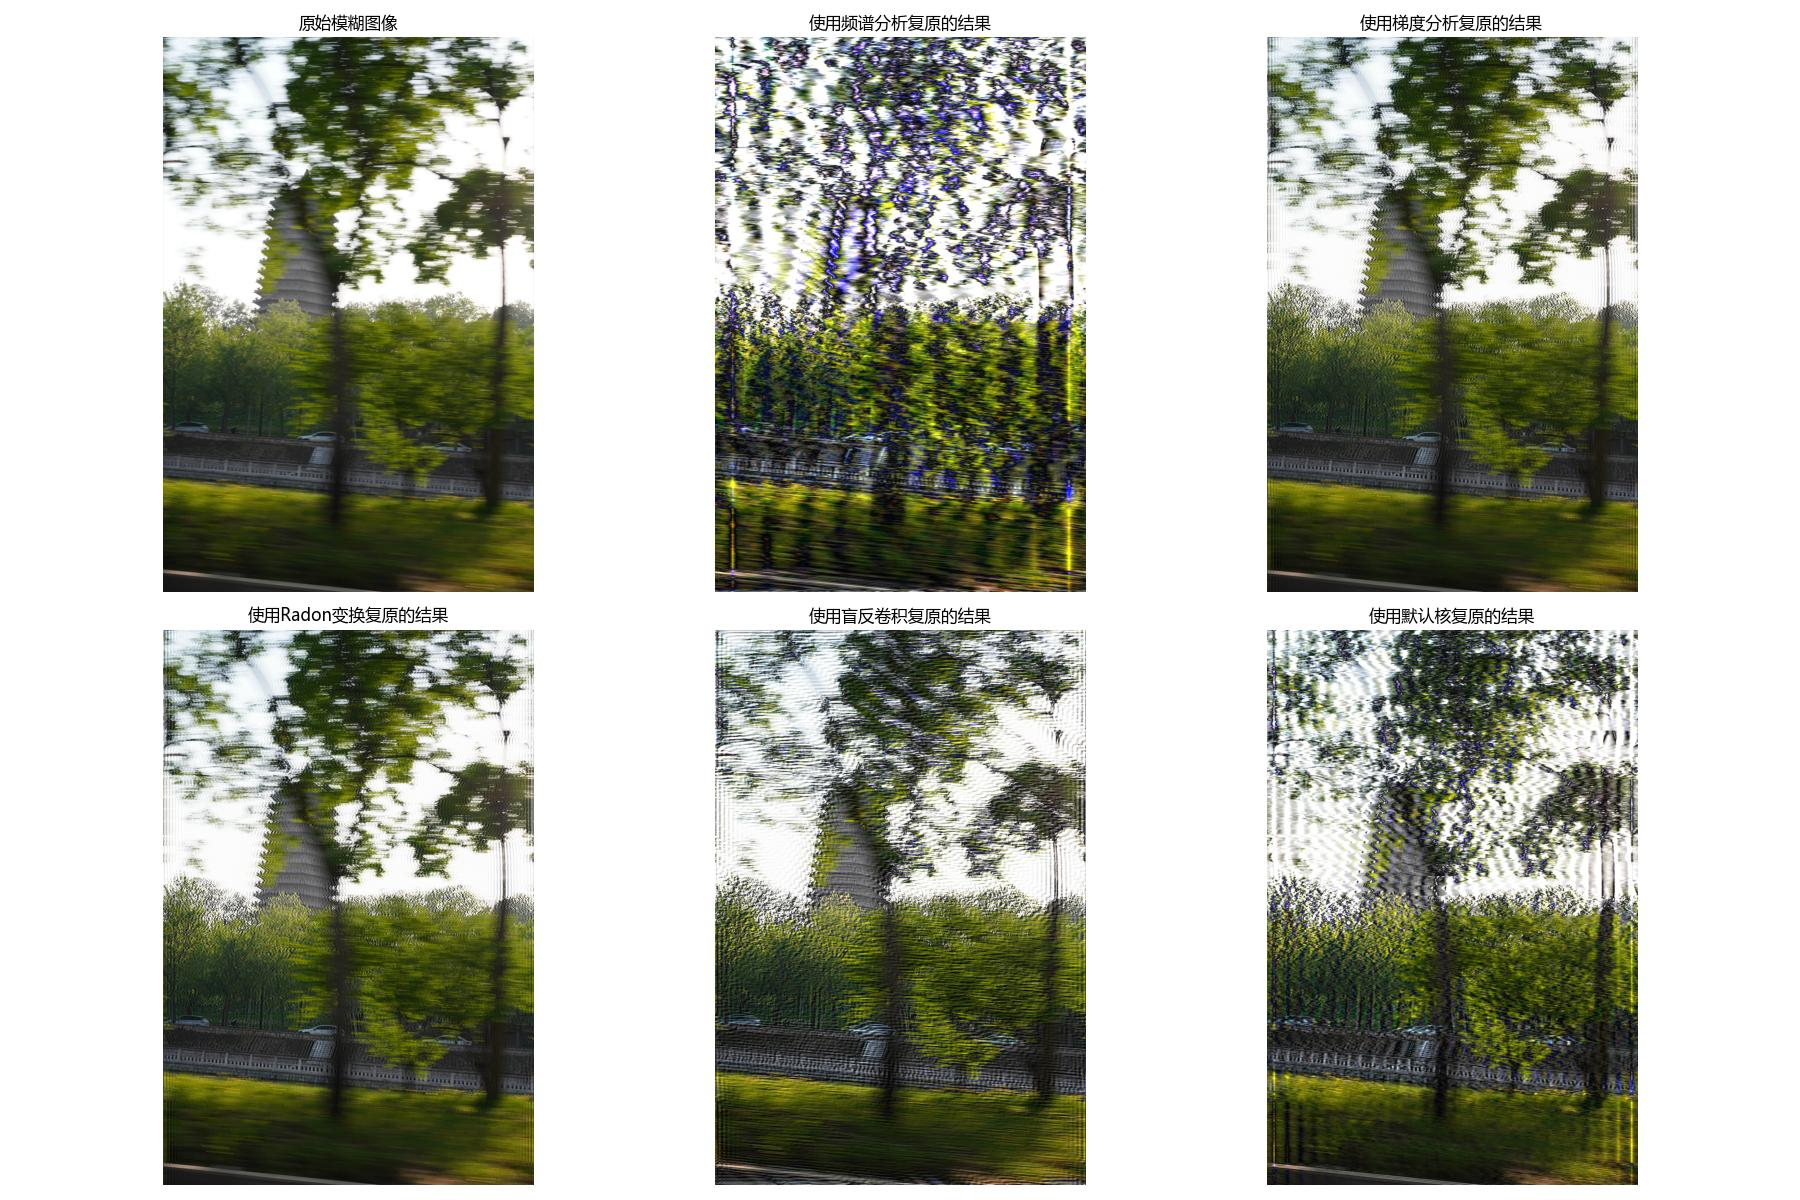
\includegraphics[width=0.9\textwidth]{2.restoration_comparison.jpg}
  \caption{使用不同模糊核复原的结果对比}
\end{figure}

本实验采用的原始图像是在运动的汽车上拍摄，由于包含不同距离的景物，它们的模糊程度因此有很大差异。表现为近处的物体较为模糊，远处的物体不算模糊。这种模糊程度的差异，导致使用同一种去模糊的核不能在所有的场景下表现良好。

在所有的复原图像上都出现了不同程度的波纹，这是由于模糊核估计不正确导致的，估计偏差越大，对应的波纹越大。
具体分析每种办法，从图2可以看出：
\begin{itemize}
    \item 频谱分析法：复原效果最差，出现断裂的色彩。原因可能是在进行频域变换的时候有除法操作，导致某些频率分量放大，也有可能是RGB的放大比例不同而导致的色差失真。
    \item 梯度分析法：复原效果最好，边缘清晰度提高。因此可以得知，梯度方法在分析规律运动模糊的情况下效果较好。
    \item Radon变换法：估计核一致，复原效果最好。
    \item 盲反卷积法：复原效果较好。
    \item 默认核（长度15，角度0度）：由于错误估计长度，在和梯度方法一致的情况下，复原效果出现了明显的波纹。
\end{itemize}

\begin{figure}[htbp]
  \centering
  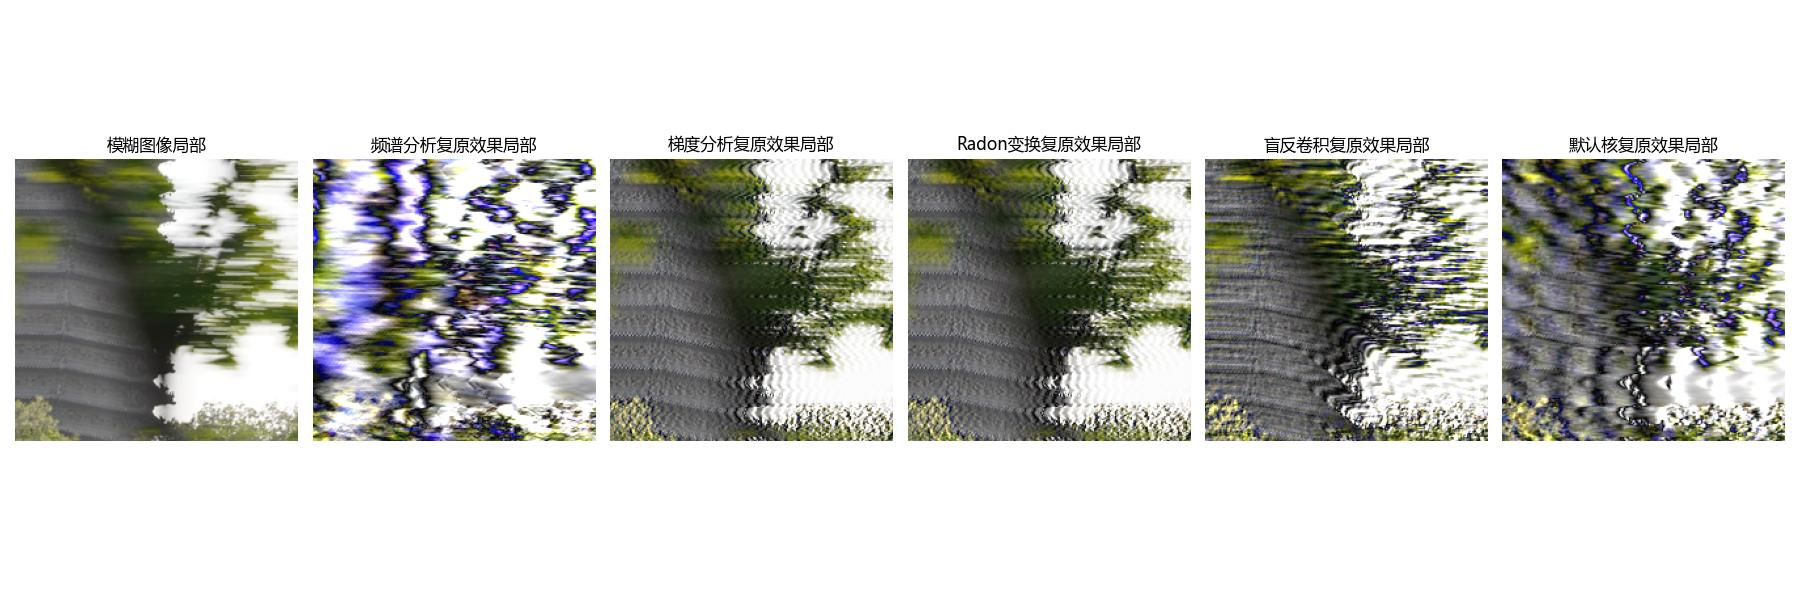
\includegraphics[width=0.9\textwidth]{2.detail_comparison.jpg}
  \caption{局部细节对比}
\end{figure}

图3展示了局部区域的复原效果对比。从细节放大可以更清晰地看出各方法的差异：
\begin{itemize}
    \item Radon变换法和梯度分析法在细节复原上表现较好，能够恢复更多的纹理信息。
    \item 频谱分析法和默认核效果最差，出现色彩伪影。
    \item 盲反卷积由于错误估计角度，导致水平和垂直方向均出现波纹。
\end{itemize}

\begin{figure}[htbp]
  \centering
  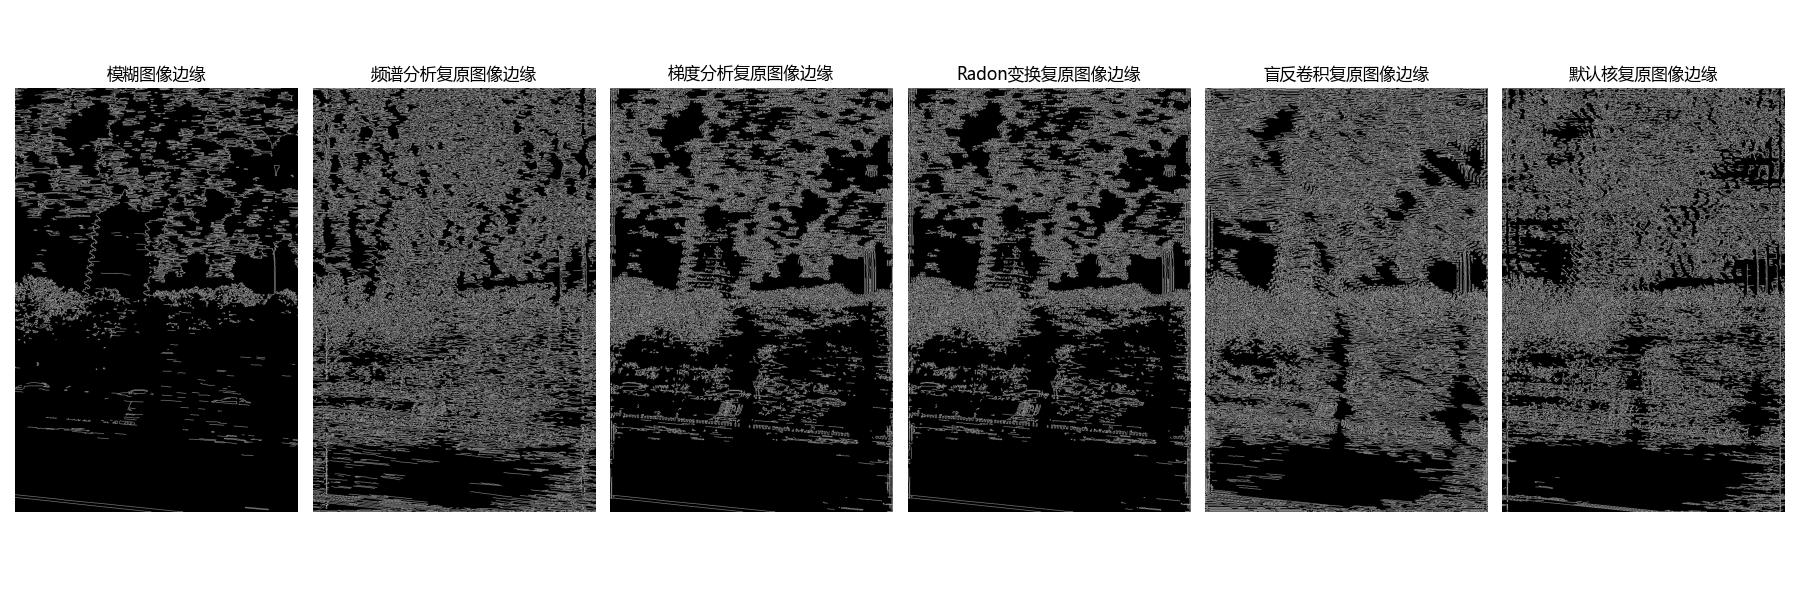
\includegraphics[width=0.9\textwidth]{2.edge_comparison.jpg}
  \caption{边缘质量对比}
\end{figure}

图4展示了各方法复原图像的边缘检测结果。边缘的清晰度和连续性是衡量复原质量的重要指标：
\begin{itemize}
    \item 梯度分析法和Radon变换法复原的边缘最为清晰和连续。
    \item 盲反卷积法,频谱分析法复原的边缘最差。
\end{itemize}

\subsection{评估指标比较}

\begin{figure}[htbp]
  \centering
  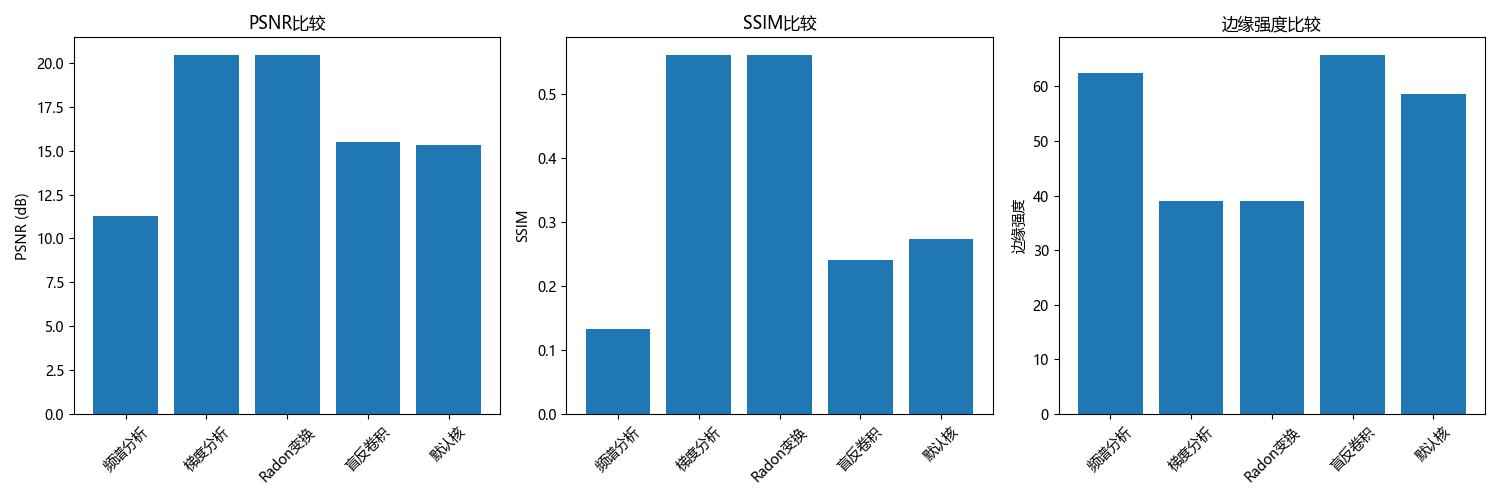
\includegraphics[width=0.9\textwidth]{2.metrics_comparison.jpg}
  \caption{不同方法的评估指标对比}
\end{figure}

图5展示了不同复原方法的三个评估指标：PSNR（峰值信噪比）、SSIM（结构相似性）和边缘强度。从图中可以看出：

\begin{itemize}
    \item PSNR方面，梯度分析法和Radon变换法表现较好，说明它们复原的图像在像素级别与原图较为接近
    \item SSIM方面，梯度分析法和Radon变换法得分较高，表明它们在保持图像结构特性方面更为出色
    \item 边缘强度方面，盲反卷积法高于其他方法，说明它们复原的图像边缘更为清晰，但是和观感上效果不好
\end{itemize}

\begin{table}[htbp]
    \caption{不同分析方法的性能指标对比}
    \centering
    \begin{tabular}{lccc}
        \toprule
        分析方法 & PSNR & SSIM & 边缘强度 \\
        \midrule
        频谱分析 & 11.28dB & 0.1334 & 62.4141 \\
        梯度分析 & 20.43dB & 0.5602 & 38.9909 \\
        Radon变换 & 20.43dB & 0.5602 & 38.9909 \\
        盲反卷积 & 15.50dB & 0.2409 & 65.6955 \\
        默认核 & 15.35dB & 0.2738 & 58.5552 \\
        \bottomrule
    \end{tabular}
\end{table}


\subsection{参数自动调优结果}

实验还尝试了自动调整维纳滤波的K参数，以获得最佳复原效果。结果显示：

\begin{itemize}
  \item 频谱分析 的最佳K值: 0.001, 得分: 232.2057
  \item 梯度分析 的最佳K值: 0.001, 得分: 195.4505
  \item Radon变换 的最佳K值: 0.001, 得分: 195.4505
  \item 盲反卷积 的最佳K值: 0.001, 得分: 255.9062
  \item 默认核 的最佳K值: 0.001, 得分: 240.5433
\end{itemize}

根据综合评分，盲反卷积法配合K=0.001的维纳滤波参数取得了最佳复原效果。但是这和感官上不符合。感官最好的反而评分更低。

\section{总结及心得体会:}
通过本次实验，我深入理解了模糊图像复原的基本原理和方法，尤其是维纳滤波和不同模糊核估计方法的特点。 模糊核的准确估计对复原效果至关重要，不同的估计方法有各自的优缺点。如果知道原始图像的运动规律，那么选择对应的模糊估计函数会起到很大作用。

\vspace{4cm}
\begin{flushright}
\begin{tabular}{lc}
\sihao{\hei{报告评分：}}& \sihao{\vspace{10pt}}\\
\sihao{\hei{指导教师签字：}}& \sihao{\vspace{10pt}}\\
\end{tabular}
\end{flushright}


\end{document}
